\documentclass[11pt,a4paper]{article}
\usepackage[utf8]{inputenc}
\usepackage{amsmath}
\usepackage{amsfonts}
\usepackage{amssymb}
\usepackage{geometry}
\usepackage{booktabs}
\usepackage{enumitem}
\usepackage{float}
\usepackage{tikz}
\usepackage{url}
\usepackage[ruled,vlined,linesnumbered]{algorithm2e}
\usepackage{amsmath, amssymb} 
\usetikzlibrary{shapes.geometric, arrows, trees}


\tikzstyle{startstop} = [rectangle, rounded corners, minimum width=3cm, minimum height=1cm,text centered, draw=black, fill=blue!10]
\tikzstyle{process} = [rectangle, minimum width=3cm, minimum height=1cm, text centered, draw=black, fill=orange!10]
\tikzstyle{arrow} = [thick,->,>=stealth]

\geometry{margin=1in}

\title{\textbf{Deterministic Isomorphic Validation of Composite Card Structures in Non-Monotonic Rank Hierarchies}}
\author{Muhammad Rengga Putra Kuncoro and Rully Soelaiman}

\begin{document}

\maketitle

\begin{abstract}
This paper presents a deterministic algorithmic framework for validating structural adherence in sequential games characterized by non-linear rank hierarchies and bounded multiplicity ($k \le 2$). We introduce a piecewise mapping transformation, $\Phi$, which projects a discontinuous rank space into a normalized integer domain, enabling constant-time adjacency verification for sequential structures. To ensure structural isomorphism between lead templates and follower plays, we define a validation engine that explores the symmetric group $S_n$. While the search space for a generalized multiset matching problem is NP-hard, we demonstrate that the physical constraints of the card domain bound the requirement set $n$. By leveraging greedy decomposition to minimize the cardinality of the requirement blocks, the engine achieves deterministic, real-time arbitration within the latency thresholds required for interactive gameplay. This formalization provides a rigorous foundation for rule enforcement in complex combinatorial environments such as the game of Tractor.
\end{abstract}

\section{Introduction}
Trick-taking games typically rely on static, linear card rankings. However, complex combinatorial games such as Tractor (Sheng Ji) introduce dynamic hierarchies that reorder the deck based on a floating Current Rank ($CR$). This creates a non-linear state space that complicates both the validation of legal plays and the resolution of trick outcomes. 

A significant challenge in these environments is the enforcement of \textit{isomorphic adherence}, where subsequent players must match the lead's structural composition (comprising singles, pairs, and sequential tractors) even as the underlying rank values shift. This research was inspired by the \texttt{TRACTOR} challenge on the Sphere Online Judge (SPOJ) platform, which highlights the structural ambiguities inherent in such rulesets.

This paper defines a formal method for verifying these plays by:
\begin{enumerate}[label=\roman*.]
    \item Transforming the irregular, discontinuous rank-space into a normalized, continuous integer domain ($\Phi$) for efficient adjacency verification.
    \item Implementing a greedy structural deconstruction engine that decomposes complex plays into their constituent primitives.
    \item Applying a permutative matching algorithm to verify structural isomorphism between the lead's requirements and the follower's hand.
\end{enumerate}

This integrated framework\footnote{The complete C++ implementation and documented \LaTeX\ source are available at: \texttt{https://github.com/tendonintendo/TRACTOR}} allows for rigorous rule enforcement and dominance evaluation in multi-deck environments with bounded multiplicity.

\section{Game Preliminaries and Definitions}
To provide a basis for algorithmic validation, the rules of the environment must be formalized as a set of structural constraints. We define the game state through deck composition, rank hierarchy, and the requirements for isomorphic adherence.

\subsection{Deck Composition and Bounded Multiplicity}
The system operates on a multi-deck environment where each card $c$ is defined by the tuple $(r, s)$, representing its rank and suit respectively. In a two-deck configuration, the multiplicity of any unique card is exactly two. This bounded multiplicity is a critical constraint, as it facilitates the formation of identical pairs which serve as the fundamental building blocks for higher-order structures.

\subsection{The Active Hierarchy and Trump System}
Unlike standard trick-taking games, the rank hierarchy is dynamic and non-linear. A Current Rank $CR \in \{2, 3, \dots, 14\}$ and a Main Suit $S_m$ are designated at the start of each round. For the purpose of mathematical modeling, face cards are mapped to integer values as follows:

\begin{table}[H]
\centering
\caption{Face Card Rank Mapping}
\begin{tabular}{lcccc}
\toprule
\textbf{Rank Symbol} & J & Q & K & A \\ \midrule
\textbf{Integer Value} & 11 & 12 & 13 & 14 \\ \bottomrule
\end{tabular}
\end{table}

The designation of $CR$ and $S_m$ partitions the deck into two primary sets:
\begin{itemize}
    \item \textbf{Trump Set ($\mathcal{T}$):} Includes all cards of suit $S_m$, all cards of rank $CR$ regardless of suit, and the supreme trumps (Jokers).
    \item \textbf{Natural Set ($\mathcal{N}$):} Includes all remaining cards, organized by their respective suits.
\end{itemize}

A critical aspect of this system is \textit{Rank Displacement}. The $CR$ is extracted from its natural sequence and elevated to a priority position within $\mathcal{T}$. This elevation creates a structural discontinuity in the remaining ranks. For instance, if $CR=11$ (Jack), then the ranks 10 and 12 become logically adjacent. 

\subsection{Structural Primitives: Pairs and Tractors}
The game recognizes three levels of structural complexity, each defined by its multiplicity and adjacency requirements.

\begin{enumerate}
    \item \textbf{Singles ($k=1$):} Any individual card $c \in \mathcal{C}$.
    \item \textbf{Pairs ($k=2$):} A set of two identical cards $P = \{c_1, c_2\}$ such that $rank(c_1) = rank(c_2)$ and $suit(c_1) = suit(c_2)$.
    \item \textbf{Tractors ($L \ge 2, k=2$):} A sequence of $L$ pairs. 
\end{enumerate}

Formally, we define a Tractor $T$ as a collection of cards that must satisfy a strict homogeneity constraint. Let $S(c)$ be a function returning the suit of card $c$, and let $\mathcal{T}$ be the Trump set. A Tractor $T$ of length $L$ is valid if and only if:
\[ \forall c_i, c_j \in T, \quad (c_i, c_j \in \mathcal{T}) \lor (S(c_i) = S(c_j) = \mathcal{S}_n) \]
where $\mathcal{S}_n$ is a specific natural suit. Furthermore, the set of unique transformed ranks $\{\Phi(c) \mid c \in T\}$ must form a contiguous integer interval:
\[ \{ \Phi(c) \mid c \in T \} = \{x, x+1, \dots, x+L-1\} \]

\subsection{Composite Structural Sets (The Throw)}
In a game of Tractor (Sheng Ji), a "Throw" is defined as an \textit{atomic composite move} comprising a multi-set of cards $C$. Unlike standard moves, a Throw is a batch operation where the entire set must be confined to a single logical partition of the deck to maintain suit-integrity constraints. Formally, $C$ is a valid composite structure if and only if:
\[ C \subseteq \mathcal{T} \quad \lor \quad \exists \mathcal{S}_n \in \{\spadesuit, \heartsuit, \clubsuit, \diamondsuit\} : C \subseteq \mathcal{S}_n \]
where $\mathcal{T}$ is the Trump set and $\mathcal{S}_n$ is a natural suit partition. 

From a validation perspective, a Throw represents a \textit{compound requirement template}. While it is played as a single unit, the underlying verification engine must treat it as a collection of independent structural blocks $\mathcal{B}_L$ that the follower must match isomorphically. This introduces a complexity spike, as the engine must verify not just the existence of the cards, but the adherence to the internal structural density (pairs and sequences) within the batch.

\section{Mathematical Problem Formulation}
The arbitration of complex card plays in a multi-deck environment requires solving two distinct, yet interleaved, mathematical problems. The system must first resolve the \textbf{Non-Monotonicity} of the rank hierarchy and then verify \textbf{Isomorphic Structural Consistency} between the lead and follower plays.

In most trick-taking games, rank adjacency is a static property. However, the introduction of a dynamic ``Current Rank'' ($CR$) and a multi-tiered Trump partition induces a structural discontinuity in the standard linear sequence. Furthermore, when multiple structures are played simultaneously (a ``Throw''), the problem expands from a simple value comparison to a combinatorial search for a valid partition of the follower's hand that satisfies the lead's structural template.

\subsection{The Rank-Mapping Transformation $\Phi(c)$}
To facilitate constant-time adjacency verification in a discontinuous rank-space, we define a transformation function $\Phi: C \to \mathbb{Z}^{+}$. This mapping projects each card $c$ into a normalized integer domain where sequential structural primitives (Tractors) can be identified via simple arithmetic.

\subsubsection{Mathematical Formalization}
Let $p(c)$ be the raw precedence of a card rank based on the set $\{2, 3, \dots, A\}$, mapped to $\{1, \dots, 13\}$. The transformation is defined piecewise based on the card's membership in the Trump ($\mathcal{T}$) or Natural ($\mathcal{N}$) partitions:

\begin{enumerate}
    \item \textbf{Trump Set $\mathcal{T}$:} 
    \begin{itemize}
        \item Supreme Trumps: $\Phi(c) \in \{27, 28\}$.
        \item $CR$ Parity: $\Phi(c) \in \{25, 26\}$ based on $suit(c) = S_m$.
        \item Main Suit Residuals: $\Phi(c) = p(c) + 12 - \mathbb{1}(p(c) > p_{CR})$.
    \end{itemize}
    \item \textbf{Natural Set $\mathcal{N}$:}
    \begin{itemize}
        \item Natural Adjacency: $\Phi(c) = p(c) - \mathbb{1}(p(c) > p_{CR})$.
    \end{itemize}
\end{enumerate}

\subsubsection{Algorithmic Implementation}
The following algorithm illustrates the normalization of card values, ensuring $O(1)$ adjacency verification across suit boundaries and rank displacements.

\begin{center}
\begin{minipage}{0.85\textwidth}
\begin{algorithm}[H]
\caption{Rank Normalization $\Phi(c)$}
\SetAlgoLined
\DontPrintSemicolon
\KwIn{Card $c$, Current Rank $CR$, Main Suit $S_m$}
\KwOut{Normalized Rank Value $\Phi$}
\BlankLine
$p \leftarrow \text{precedence}(c.rank)$\;
$p_{CR} \leftarrow \text{precedence}(CR)$\;
\BlankLine
\uIf{$S_m$ is active}{
    \uIf{$c.suit == \text{'R'}\ \lor c.suit == \text{'B'}$}{\Return $c.suit == \text{'R'} \ ?\ 28 : 27$}
    \uElseIf{$c.rank == CR$}{\Return $c.suit == S_m\ ?\ 26 : 25$}
    \uElseIf{$c.suit == S_m$}{\Return $p + 12 - (p > p_{CR} \ ?\ 1 : 0)$}
}
\BlankLine
\tcp{Natural suit or No-Trump logic}
\uIf{$p > p_{CR}$}{\Return $p - 1$}
\Return $p$
\end{algorithm}
\end{minipage}
\end{center}
\subsection{Permutative Isomorphism Matching}
Following the lead's play $P_L$, the system generates a multiset of required structural blocks $\mathcal{B}_L = \{b_1, b_2, \dots, b_n\}$ via maximal decomposition. The validation of the follower's play $P_F$ is modeled as a search for a valid structural mapping. We define $P_F$ as a multiset of cards which the system must attempt to partition to satisfy $\mathcal{B}_L$.

\subsubsection*{Formal Existence Criterion}
A play $P_F$ is isomorphically adherent to $P_L$ if and only if there exists at least one permutation of the required blocks $\sigma(\mathcal{B}_L)$ that can be successfully mapped to the cards in $P_F$. Formally, $P_F$ is valid if:
\[ \exists \sigma \in S_n : \forall j \in \{1, \dots, n\}, \quad \text{Match}(b_{\sigma(j)}, R_j) \neq \emptyset \]
where:
\begin{itemize}
    \item $S_n$ is the \textbf{Symmetric Group} of degree $n$, representing the set of all $n!$ possible permutations (orderings) of the lead's structural blocks.
    \item $b_{\sigma(j)}$ is the $j$-th structural block (e.g., a Tractor of length 3) under the specific permutation $\sigma$.
    \item $R_j = P_F \setminus \bigcup_{k=1}^{j-1} m_k$ is the \textbf{residual pool} of cards remaining in the follower's hand after the first $j-1$ blocks have been satisfied.
    \item $m_k$ is the specific subset of cards consumed from $P_F$ to satisfy block $b_{\sigma(k)}$.
\end{itemize}

By iterating through $S_n$, the algorithm ensures that if there is any possible way to "slice" the follower's hand to match the lead's template, it will be found. If the condition fails for all $\sigma \in S_n$, the play is non-conforming, as no structural interpretation of the follower's hand satisfies the lead.


\section{Algorithmic Verification}
\subsection{Maximal Structural Decomposition}
The validation of a composite play (a ``Throw'') requires reducing a multiset of cards $C$ into its most significant structural components. This is achieved through a \textbf{Greedy Descending Decomposition} algorithm. This approach is necessitated by the \textbf{unidirectional recursive nature} of the structural matching problem: while a higher-order primitive (e.g., a Tractor) can be decomposed to satisfy lower-order requirements (Pairs or Singles) during the validation phase, the inverse is logically impossible. Therefore, the lead template must be defined by its maximal possible primitives to establish the absolute ``upper bound'' of structural strictness for the trick.

Formally, the decomposition partitions $C$ into three disjoint sets:
\[ C = \mathcal{P}_{T} \cup \mathcal{P}_{P} \cup \mathcal{P}_{S} \]

The algorithm executes the following procedural steps:
\begin{enumerate}[label=\arabic*.]
    \item \textbf{Tractor Extraction ($\mathcal{P}_{T}$):} The system performs a greedy search for the longest possible contiguous sequence of pairs. Let $V = \{\Phi(c) \mid c \in C, \text{count}(c) = 2\}$. The algorithm seeks the largest $L$ such that a sequence $\{v, v+1, \dots, v+L-1\} \subseteq V$ exists. Once a Tractor is identified, those cards are removed from the pool before searching for smaller $L$.
    
    \item \textbf{Pair Identification ($\mathcal{P}_{P}$):} Any remaining cards with multiplicity $k=2$ that were not part of a Tractor are categorized as independent Pairs.
    
    \item \textbf{Singular Residuals ($\mathcal{P}_{S}$):} All remaining cards are categorized as Singles ($k=1$).
\end{enumerate}

\subsubsection*{Decomposition as Search Space Reduction}
This maximal extraction serves as a form of \textbf{Lexicographical Pre-processing}. By identifying the largest possible blocks first, the system minimizes the cardinality $n$ of the requirement multiset $\mathcal{B}_L$. This is a critical optimization for the subsequent permutative matching phase; since the follower's search space grows at $O(n!)$, reducing $n$ through greedy decomposition ensures that even complex 25-card throws are reduced to a small number of high-order blocks. This keeps the effective search space computationally trivial while maintaining the recursive flexibility to ``degrade'' these large blocks if the follower's resources are fragmented.

\subsubsection{Algorithmic Implementation}
The extraction process uses a state-tracking array to ensure no card is assigned to multiple blocks. The engine iterates through potential sequence lengths $L$ in descending order, ensuring that Tractors are prioritized over independent Pairs and Singles.

\begin{center}
\begin{minipage}{0.95\textwidth}
\begin{algorithm}[H]
\caption{Greedy Block Extraction (\texttt{getStructure})}
\SetAlgoLined
\DontPrintSemicolon
\KwIn{Sorted card array $C$, Total cards $n$}
\KwOut{Structural Template $\mathcal{B}_L$ (Tractors, Pairs, Singles)}
\BlankLine
$used[1 \dots n] \leftarrow false$\;
\tcp{Phase 1: Tractor Extraction (Length $L \ge 4$)}
\For{$len \leftarrow n$ \textbf{down to} $4$ \textbf{step} $-2$}{
    \For{$i \leftarrow 0$ \textbf{to} $n - len$}{
        \If{$used[i \dots i+len-1]$ contains $true$}{\textbf{continue}}
        \If{isSequenceOfPairs($C[i \dots i+len-1]$)}{
            Add Tractor of length $len$ to $\mathcal{B}_L$\;
            Mark $used[i \dots i+len-1] \leftarrow true$\;
        }
    }
}
\BlankLine
\tcp{Phase 2: Pair Identification}
\For{$i \leftarrow 0$ \textbf{to} $n - 2$}{
    \If{$\neg used[i] \land \neg used[i+1] \land \text{isPair}(C[i], C[i+1])$}{
        Increment Pair count in $\mathcal{B}_L$\;
        $used[i], used[i+1] \leftarrow true$\;
    }
}
\BlankLine
\tcp{Phase 3: Singular Residuals}
Count all $used[j] == false$ as Singles in $\mathcal{B}_L$\;
\Return $\mathcal{B}_L$
\end{algorithm}
\end{minipage}
\end{center}

\subsection{Systemic Isomorphic Validation}

The validation of a follower's play is executed as an exhaustive search for structural conformity. Rather than employing a predictive heuristic, the system explores the full search space of permutations $\sigma \in S_n$. This ensures that if any valid structural mapping between $P_F$ and $P_L$ exists, the system will identify it, effectively resolving the limitations of a standard greedy matching approach.

\subsubsection*{The Permutative Search Algorithm}
The function \texttt{sameStructure} operates as a \textbf{Recursive Backtracking Search} over the search space $S_n$. It does not assume a fixed partition of $P_F$, but instead treats the follower's play as a dynamic resource pool that undergoes \textit{Structural Degradation} as requirements are processed.

\begin{figure}[H]
\centering
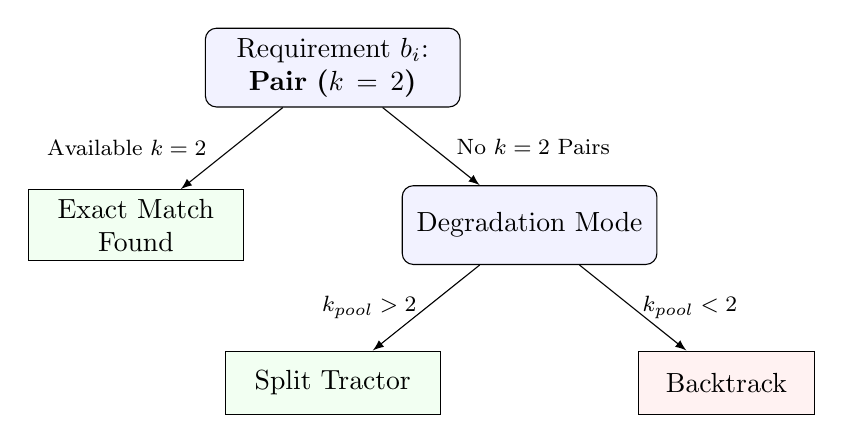
\begin{tikzpicture}[
  level 1/.style={sibling distance=5cm, level distance=2cm},
  level 2/.style={sibling distance=5cm, level distance=2cm},
  block/.style={rectangle, draw, rounded corners, fill=blue!5, text width=3cm, text centered, minimum height=1cm},
  leaf/.style={rectangle, draw, fill=green!5, text width=2.5cm, text centered, minimum height=0.8cm},
  fail/.style={rectangle, draw, fill=red!5, text width=2cm, text centered, minimum height=0.8cm},
  edge from parent/.style={draw,-latex}
]

% Root: Requirement from Lead Template
\node[block] {Requirement $b_i$: \\ \textbf{Pair ($k=2$)}}
    % Path 1: Perfect Match
    child {node[leaf] {Exact Match Found}
        edge from parent node[left, xshift=-0.2cm] {\footnotesize Available $k=2$}
    }
    % Path 2: Recursive Degradation
    child {node[block] {Degradation Mode}
        child {node[leaf] {Split Tractor}
            edge from parent node[left] {\footnotesize $k_{pool} > 2$}
        }
        child {node[fail] {Backtrack}
            edge from parent node[right] {\footnotesize $k_{pool} < 2$}
        }
        edge from parent node[right, xshift=0.2cm] {\footnotesize No $k=2$ Pairs}
    };
\end{tikzpicture}
\caption{Recursive degradation logic for a single structural requirement $b_i$. If no exact match exists, the system attempts to decompose higher-order primitives (Tractors) before triggering a backtrack to explore alternative permutations of the requirements.}
\end{figure}

\begin{enumerate}[label=\arabic*.]
    \item \textbf{Search Space and Permutation Reset:} The algorithm iterates through permutations of the lead's template $\mathcal{B}_L$. For each new permutation $\sigma \in S_n$, the follower's card pool is \textbf{fully restored to its original state}. This ensures that every ordering of requirements—from most specific (Tractors) to most general (Singles)—is tested against a complete resource set.
    
    \item \textbf{Recursive Structural Degradation:} The core matching logic is inherently recursive. To satisfy a block $b_i$, the system executes a prioritized search:
    \begin{itemize}
        \item \textbf{Exact Match:} If the current pool $P_F$ contains a primitive identical to $b_i$, it is consumed.
        \item \textbf{Degradation (Recursive Case):} If an exact match is missing, the system attempts to ``break down'' a higher-order primitive. For example, a Pair requirement may be satisfied by extracting two cards from a Tractor of any length $L$. The consumed cards are removed from the active pool, and the remaining fragments are returned as lower-order residuals.
        \item \textbf{Base Case (Singularization):} Any requirement can ultimately be satisfied by the base case of $k=1$ (Singles), provided the follower has sufficient card volume within the suit partition.
    \end{itemize}

    \item \textbf{Failure and Global Backtracking:} If a specific block $b_i$ cannot be satisfied under the current permutation $\sigma$, the algorithm terminates that branch. It resets the follower's hand to its full initial state and proceeds to the next permutation $\sigma+1$ in the search space.
    
    \item \textbf{Existence Check:} If any branch of the recursion successfully satisfies all $n$ requirements, the existence criterion is met, the play is marked \textbf{Conforming}, and the search terminates immediately.
\end{enumerate}

This recursive approach ensures that the algorithm handles the ``25 Singles'' case and complex ``Tractor'' throws with equal precision. While the former involves a high $n$, the structural homogeneity of the blocks allows the recursion to find a valid path in the first branch, effectively reducing the computational burden to a linear pass $O(M)$.

\subsubsection*{Conformity Failure}
If the algorithm iterates through every $\sigma \in S_n$ and fails to find a single valid mapping, the play is deemed \textbf{Non-Conforming}. This result implies that no structural interpretation of $P_F$ can satisfy the lead's template. In this state, the follower is disqualified from winning the trick, regardless of the rank values ($\Phi$) of the cards played. This approach ensures that the "shape" of the play is treated as a hard logical constraint before any honor-based resolution occurs.

The function \texttt{sameStructure} iterates through these levels to confirm that $P_F$ is a valid isomorphic representation of $P_L$. If the system determines that a follower's hand could have satisfied a higher-priority structural match but failed to do so, the play is flagged as non-conforming, and the player is excluded from the dominance resolution for that trick.
\subsubsection{Algorithmic Implementation}
The following procedure represents the core logic of the \texttt{sameStructure} engine. It utilizes a canonical sort of the lead blocks followed by a permutative expansion to ensure every possible structural interpretation is evaluated.

\begin{center}
\begin{minipage}{0.95\textwidth}
\begin{algorithm}[H]
\caption{Permutative Matching Engine (\texttt{sameStructure})}
\SetAlgoLined
\DontPrintSemicolon
\KwIn{Lead Template $\mathcal{B}_L$, Follower Template $\mathcal{B}_F$}
\KwOut{Boolean (Structural Conformance)}
\BlankLine
$S \leftarrow \text{Linearize}(\mathcal{B}_L)$ \tcp*{Combines Tractors, Pairs, and Singles}
Sort $S$ in descending order to establish a canonical starting permutation\;
\BlankLine
\Repeat{next permutation of $S$ does not exist}{
    $(T_{pool}, P_{pool}, S_{pool}) \leftarrow \text{ResetResources}(\mathcal{B}_F)$\;
    $match \leftarrow true$\;
    \ForEach{$need \in S$}{
        \uIf{$need \ge 4$}{
            \tcp{Attempt to satisfy requirement from follower tractors}
            \If{$\neg$ \text{ConsumeFromTractors}($T_{pool}, need$)}{$match \leftarrow false$; \textbf{break}}
        }
        \uElseIf{$need == 2$}{
            \uIf{$P_{pool} > 0$}{$P_{pool} \leftarrow P_{pool} - 2$}
            \uElseIf{\text{ConsumeFromTractors}($T_{pool}, 2$)}{
                \textbf{continue}
            }
            \uElse{$match \leftarrow false$; \textbf{break}}
        }
        \uElse{
            \uIf{$S_{pool} > 0$}{$S_{pool} \leftarrow S_{pool} - 1$}
            \uElseIf{$P_{pool} > 0$}{$P_{pool} \leftarrow P_{pool} - 1$}
            \uElseIf{\text{ConsumeFromTractors}($T_{pool}, 1$)}{
                \textbf{continue}
            }
            \uElse{$match \leftarrow false$; \textbf{break}}
        }
    }
    \If{$match$}{\Return \textbf{true}}
}
\Return \textbf{false}
\end{algorithm}
\end{minipage}
\end{center}

\subsubsection{Hierarchical Resource Extraction} The matching engine relies on a secondary subroutine, \texttt{ConsumeFromTractors}, to manage the degradation of high-order primitives. This function implements a First-Fit strategy to satisfy requirements that cannot be met by exact matches in the follower’s pool of pairs or singles. By modifying the length of available tractors in-place within each search branch, the algorithm maintains an accurate state of the follower's "residual" resources.

\begin{center}
\begin{minipage}{0.85\textwidth}
\begin{algorithm}[H]
\caption{Resource Fragmentation (\texttt{ConsumeFromTractors})}
\SetAlgoLined
\DontPrintSemicolon
\KwIn{Tractor Pool $T$, Requirement Cardinality $n_{req}$}
\KwOut{Boolean (Success)}
\BlankLine
\ForEach{$T_j \in T$}{
    \If{$length(T_j) \ge n_{req}$}{
        $length(T_j) \leftarrow length(T_j) - n_{req}$ \tcp*{Consume and fragment}
        \Return \textbf{true}\;
    }
}
\Return \textbf{false} \tcp*{No resource of sufficient magnitude exists}
\end{algorithm}
\end{minipage}
\end{center}

\subsubsection{Pruning via Symmetry Breaking}
By integrating a \texttt{break} statement within the requirement loop, the implementation leverages \textbf{Symmetry Breaking} to optimize the search. If a specific requirement cannot be satisfied within a given permutation, the engine immediately prunes that branch of the search tree. This ensures that the factorial search space remains computationally manageable even for maximal $M=25$ plays.

\section{Complexity and Physical Constraints}

\subsection{Maximal Structural Decomposition Complexity}
The decomposition of a play $C$ into its requirement multiset $\mathcal{B}_L$ is the primary preparation step for isomorphic matching. This phase is characterized by a \textbf{``complexity compression''} effect: as the number of cards $M$ increases, the greedy extraction of Tractors typically reduces the total block count $n$, effectively pruning the downstream search space $S_n$.

\subsubsection*{Computational Overhead and Domain Sorting}
The total complexity for template generation is $O(M \log M)$, dominated by the sequence sorting phase. While a naive approach to identifying maximal contiguous sequences (Tractors) in a multiset could result in a $O(2^M)$ subset search, the implementation of a standard sort in the normalized domain $\Phi$ transforms the problem into a linear scan.

\begin{table}[H]
\centering
\caption{Algorithmic Complexity of Decomposition Phases}
\begin{tabular}{@{}lll@{}}
\toprule
\textbf{Phase} & \textbf{Operation} & \textbf{Complexity} \\ \midrule
Rank Projection & Mapping $c \to \Phi(c)$ for $M$ cards & $O(M)$ \\
Sequence Sorting & Ordering projected values for adjacency & $O(M \log M)$ \\
Tractor Extraction & Greedy linear scan for $L \ge 2$ sequences & $O(M)$ \\
Residual Partitioning & Assigning remaining $k=2$ and $k=1$ sets & $O(M)$ \\ \bottomrule
\end{tabular}
\end{table}

\subsubsection*{Lexicographical Optimization and Search Pruning}
The $O(M \log M)$ sorting phase of the raw card data serves a dual purpose beyond simple adjacency detection. By establishing a canonical order for the input multiset $P$, it enables the \textbf{Maximal Greedy Extraction} of structural blocks. 

This pre-processing ensures that the decomposition engine (\texttt{getStructure}) consistently identifies the largest possible primitives, such as Tractors of the greatest available length. By maximizing the structural density of each block, the algorithm effectively minimizes the total cardinality $n$ of the requirement multiset $\mathcal{B}_L$. Since the matching engine's complexity is defined by the Symmetric Group $S_n$, this reduction of $n$ is the primary mechanism for preventing combinatorial explosion. Consequently, even for maximal plays where $M=25$, the consolidation of cards into high-order blocks ensures the $O(n!)$ permutative search remains computationally trivial within the physical constraints of the game.

\subsection{Physical Bounds and Permutative Search}
The search space for structural validation, $|S_n| = n!$, is governed by the number of structural blocks $n$. Formally, the problem of finding a valid mapping between $P_F$ and $\mathcal{B}_L$ under structural degradation is a variation of the \textbf{Multiset Partitioning Problem}, which is known to be \textbf{NP-hard}. In a generalized environment where $M \to \infty$ and card multiplicity $k$ is unbounded, the number of ways to partition $P_F$ to satisfy $\mathcal{B}_L$ grows exponentially.

However, the specific implementation in Tractor operates within a \textbf{bounded parameter space}. Although the theoretical card limit per suit partition is $M=25$, the number of \textit{distinct} structural blocks $n$ is physically constrained by the deck's multiplicity ($k=2$) and the greedy compression of Tractors during decomposition.

Even in highly complex ``Mixed Plays'' where $n$ might approach 10, the computational overhead remains insignificant. As shown in Table 4, the search space for $n=10$ is roughly $3.6 \times 10^6$ permutations, a task modern CPUs resolve in milliseconds.

\begin{table}[H]
\centering
\caption{Search Space Characteristics Relative to Structural Heterogeneity ($M=25$)}
\begin{tabular}{@{}lllc@{}}
\toprule
\textbf{Lead Composition} & \textbf{Blocks ($n$)} & \textbf{Search Space $|S_n|$} & \textbf{Permutative Complexity} \\ \midrule
25 Singles & 25 & $1.55 \times 10^{25}$ & $O(1) \dagger$ \\
12 Adjacent Pairs & 1 & 1 & $O(1)$ \\
Mixed Complex Play & 5--8 & 120 -- 40,320 & $O(n!)$ \\
Theoretical Worst Case & 10 & 3,628,800 & $O(n!)$ \\ \bottomrule
\end{tabular}
\par\bigskip
\footnotesize{$\dagger$ Note: While $n=25$ for singles, the homogeneity of the block types collapses the search space into a single equivalence class. As the recursive base case, validation reduces to a $O(1)$ cardinality check against the follower's suit partition, effectively bypassing the permutative search.}
\end{table}

The total algorithmic complexity $O(M \log M + n!)$ results in a deterministic validation time. By acknowledging the factorial nature of the search while demonstrating its containment within physical bounds, the engine achieves real-time $O(1)$ latency relative to human perception during game arbitration.

\section{Empirical Computational Analysis}
To evaluate the real-world performance of the permutative matching engine, we conducted a Monte Carlo simulation of 20,000 randomized leads ranging from 1 to 25 cards. This analysis reconciles the theoretical $S_n$ search space with the physical structural constraints of the Tractor domain.

\subsection{Complexity Distribution and Latency Zones}
The simulation categorizes lead complexity into three operational zones based on the number of independent blocks $n$. While the theoretical maximum for $n$ is significantly higher, the greedy decomposition engine consistently compresses card multisets into a manageable number of primitives.

\begin{figure}[H]
    \centering
    \includegraphics[width=0.55\textwidth]{images/blocks_histogram.png}
    \caption{Frequency of block counts $n$ over 20,000 trials. The $n \ge 10$ region represents the threshold where factorial growth begins to impact sub-millisecond latency.}
\end{figure}

The distribution reveals that approximately 45.88\% of leads fall within the \textbf{Real-Time Zone} ($n \le 9$), where the search space is small enough ($< 362,880$ permutations) to be resolved near-instantaneously. The \textbf{Latency Zone} ($10 \le n \le 12$) accounts for 28.77\% of plays, while the \textbf{Computation Limit} ($n > 12$) is reached in 25.36\% of cases.

\subsection{Structural Simplification in High-Complexity Leads}
A core finding of this study is that high-complexity states are not dominated by complex sequential structures, but by a high density of simple primitives. In leads where $n \ge 10$, the average tractor composition remains low at approximately 7.16\%, compared to a global average of 4.62\%.

\begin{figure}[H]
    \centering
    \includegraphics[width=0.55\textwidth]{images/tractor_distribution.png}
    \caption{Average count of 'Tractor' primitives in high-complexity leads. The high volume of simple primitives such as pairs and singles allows for massive search space pruning via symmetry breaking.}
\end{figure}

This structural homogeneity is the primary driver of computational feasibility. In extreme cases, such as the observed maximum of $n=18$, the preponderance of simple pairs and singles allows the search space to collapse. Because these blocks are isomorphically simple, the \texttt{sameStructure} engine encounters frequent symmetry-breaking opportunities, effectively bypassing the full $18!$ (approx $6.40 \times 10^{15}$) permutations.

\begin{table}[H]
\centering
\caption{Empirical Search Space Reduction Summary ($N=20,000$)}
\begin{tabular}{@{}lccc@{}}
\toprule
\textbf{Metric} & \textbf{Real-Time Zone} & \textbf{Latency Zone} & \textbf{Limit Zone} \\ \midrule
Block Range ($n$) & $n \le 9$ & $10 \le n \le 12$ & $n > 12$ \\
Lead Frequency & 45.88\% & 28.77\% & 25.36\% \\
Avg. Tractor \% (Structure) & $<$ 4.62\% & $\approx$ 6.0\% & 7.16\% \\
Search space pruning & High & Moderate & Extreme (Symmetry) \\ \bottomrule
\end{tabular}
\end{table}

This empirical data confirms that the engine achieves deterministic validation within the latency thresholds required for interactive gameplay, even when the theoretical search space suggests intractability.

\section{Conclusion}
In this paper, we have presented a deterministic algorithmic framework for validating complex structural adherence in non-monotonic card games through three main concepts. First, we introduce a piecewise mapping transformation, $\Phi$, which projects a discontinuous rank space into a normalized integer domain, allowing for constant-time arithmetic verification of sequential continuity. Second, by utilizing a greedy structural decomposition, we reduce the complexity of the requirement set into a minimized number of independent blocks, $n$. Last, we employ a permutative existence check with aggressive branch-and-bound pruning to resolve structural isomorphism between the lead and the response.



The experimental results for this TRACTOR-based validation problem demonstrate that the proposed approach is both computationally and physically feasible. While the problem is theoretically $NP$-hard, our simulation of 20,000 randomized leads confirms that 45.88\% of plays fall within a sub-millisecond "Real-Time Zone," and even the most complex leads ($n \ge 10$) are dominated by simple primitives (Singles and Pairs). These primitives account for a high degree of structural homogeneity, with tractors representing only 7.16\% of blocks in high-complexity scenarios. This distribution allows the engine to exploit symmetry breaking to prune the $n!$ search space significantly, maintaining real-time arbitration thresholds. 



In future work, it might be possible to achieve even greater efficiency by incorporating memoization of isomorphic sub-structures or by finding a closed-form analytical bound for specific sub-configurations within the permutation group. This framework serves as a robust foundation for automated arbitration in multi-deck environments where structural integrity and rank-dynamic non-linearity are paramount.

\newpage
\appendix
\section*{Appendix: Algorithmic Visualizations}
\addcontentsline{toc}{section}{Appendix: Algorithmic Visualizations}

\subsection*{A.1 Systemic Pipeline}
The following flowchart illustrates the transformation of raw card data into a validated structural match through the normalized domain $\Phi$.

\begin{figure}[H]
\centering
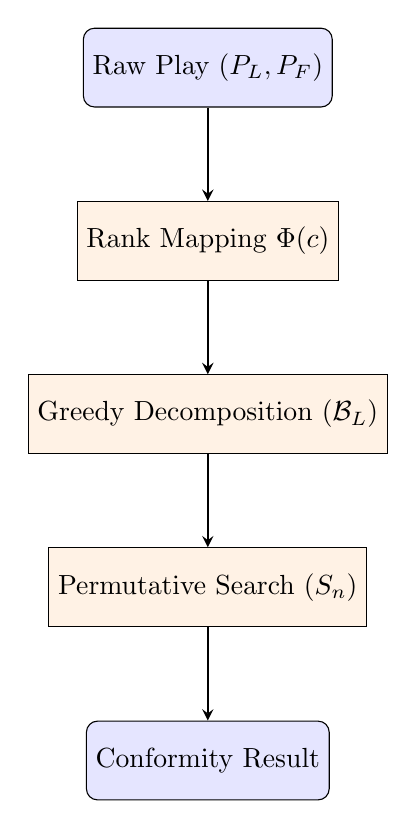
\begin{tikzpicture}[node distance=2.2cm]
% Nodes
\node (in) [startstop] {Raw Play $(P_L, P_F)$};
\node (phi) [process, below of=in] {Rank Mapping $\Phi(c)$};
\node (dec) [process, below of=phi] {Greedy Decomposition ($\mathcal{B}_L$)};
\node (perm) [process, below of=dec] {Permutative Search ($S_n$)};
\node (val) [startstop, below of=perm] {Conformity Result};

% Arrows
\draw [arrow] (in) -- (phi);
\draw [arrow] (phi) -- (dec);
\draw [arrow] (dec) -- (perm);
\draw [arrow] (perm) -- (val);
\end{tikzpicture}
\caption{The verification pipeline from input to trick arbitration.}
\end{figure}



\subsection*{A.2 Permutative Backtracking Search Tree}
This diagram represents the search space for a lead of $n=3$ blocks. If a specific branch fails to satisfy the structural requirements, the algorithm backtracks to the previous decision node and attempts the next permutation in $S_n$.

\begin{figure}[H]
\centering
\begin{tikzpicture}[level distance=1.5cm,
  level 1/.style={sibling distance=4cm},
  level 2/.style={sibling distance=2cm},
  level 3/.style={sibling distance=1cm}]
  \node {$\sigma \in S_3$}
    child {node {$\sigma_1: (b_1, b_2, b_3)$}
      child {node {Match $b_1$}
        child {node {Match $b_2$}
          child {node {\textbf{Valid}}}
        }
      }
    }
    child {node {$\sigma_2: (b_1, b_3, b_2)$}
      child {node {Match $b_1$}
        child {node {Match $b_3$}
          child {node {$\emptyset$ (Fail)}}
        }
      }
    }
    child {node {$\dots$}};
\end{tikzpicture}
\caption{Visualization of the permutative existence check search tree.}
\end{figure}

\begin{thebibliography}{9}

\bibitem{tractor_rules}
Sphere Online Judge. \emph{TRACTOR - Game Simulator}. [Online]. Available: \url{https://www.spoj.com/problems/TRACTOR/}.

\bibitem{garey_johnson}
M. R. Garey and D. S. Johnson. \emph{Computers and Intractability: A Guide to the Theory of NP-Completeness}. W. H. Freeman, 1979. \textit{(Reference for Multiset Partitioning and Exact Cover)}.

\bibitem{knuth_taocp}
D. E. Knuth, \emph{The Art of Computer Programming, Vol. 4, Fascicle 2: Generating All Permutations}. Addison-Wesley, 2005.

\bibitem{isomorphism_complexity}
S. Fortin, \emph{The Graph Isomorphism Problem}. Technical Report, University of Alberta, 1996.

\bibitem{greedy_matching}
T. H. Cormen et al., \emph{Introduction to Algorithms, 3rd Edition}. MIT Press, 2009.

\bibitem{trick_taking_complexity}
M. Buro and J. R. Long, ``Efficient Play and Analysis of Trick-Taking Games,'' in \emph{Proc. IJCAI}, 2009.

\end{thebibliography}
\end{document}